\documentclass[conference]{IEEEtran}

% ---------- Packages ----------
\usepackage{cite}
\usepackage{amsmath,amssymb}
\usepackage{tikz}
\usetikzlibrary{arrows.meta,positioning,fit,shapes.misc,shapes.symbols}
\usepackage{pgfplots}
\pgfplotsset{compat=1.18}
\usepackage{xcolor}
\usepackage{float}
\usepackage[compact]{titlesec}

% --- tighten section spacing ---
\titlespacing{\section}{0pt}{*1.3}{*0.6}
\titlespacing{\subsection}{0pt}{*1.0}{*0.5}
\titlespacing{\subsubsection}{0pt}{*0.8}{*0.4}

% ---------- Document ----------
\begin{document}

\title{FeFET CMOS 0.18~$\mu$m Integration Study}

\author{\IEEEauthorblockN{Shinichi Samizo}
\IEEEauthorblockA{Independent Semiconductor Researcher; Former Engineer at Seiko Epson Corporation\\
Email: shin3t72@gmail.com, GitHub: https://github.com/Samizo-AITL}
}

\maketitle

\begin{abstract}
Ferroelectric field-effect transistors (FeFETs) based on Hf$_{0.5}$Zr$_{0.5}$O$_2$ (HZO) provide a CMOS-compatible option for embedded non-volatile memory (NVM). We demonstrate the integration of a gate-last FeFET module into a legacy 0.18~$\mu$m CMOS logic baseline with only one additional mask step. Fabricated devices exhibit a threshold-window of 0.8--1.0~V, endurance beyond $10^5$ program/erase cycles, and retention exceeding 10 years at 85$^\circ$C by Arrhenius projection. These features enable instant-on operation, SRAM backup, and secure key storage in automotive/IoT applications using mature 0.18~$\mu$m technology.
\end{abstract}

\begin{IEEEkeywords}
FeFET, HfZrO$_2$, 0.18~$\mu$m CMOS, reliability, process integration
\end{IEEEkeywords}

% ---------------- Main Body ----------------
\section{Introduction}
FeFETs based on HZO thin films have emerged as a CMOS-compatible option for embedded NVM~\cite{Boscke2011,Mueller2012,Schenk2019}. We target a legacy 0.18~$\mu$m CMOS flow and demonstrate a minimal-overhead integration of FeFET modules. This paper makes three contributions: (i) drop-in FeFET module fully compatible with the baseline logic flow, (ii) realization with only one extra mask (cost minimization), and (iii) quantitative evaluation of endurance/retention. Surveys of FeFET integration/reliability appear in~\cite{Mueller2015,Park2020}, and automotive reliability considerations in~\cite{Nakamura2003}.

\section{Process Integration}
\subsection{Flow Placement (Fig.~\ref{fig:flow})}
The ferroelectric (FE) gate stack is inserted after polysilicon definition. Only one additional mask is required.

\subsection{Device Stack and Notes}
TiN / Hf$_{0.5}$Zr$_{0.5}$O$_2$ (8--12~nm, ALD) / Al$_2$O$_3$ interfacial layer (1--2~nm) / p-Si. Notes: The 1.8~V/3.3~V baseline is extended with an 1.8~V FeFET option. FeFETs serve as auxiliary NVM blocks for 1.8~V SRAM macros (not large arrays). Integration is feasible in a 0.18~$\mu$m line by adding ALD; TiN can reuse barrier sputter tools. The FeFET module is inserted after FEOL Co salicide and lamp anneal, requiring only one extra mask.

\section{Experimental Conditions}
To represent the \textbf{newly added FeFET capacitor option} in the 0.18~$\mu$m flow, MIM-like capacitors using the same IL/FE/TiN stack were fabricated and used as a reliability vehicle. Unless noted, the following conditions apply:
\begin{itemize}
  \item \textbf{FE gate stack:} Hf$_{0.5}$Zr$_{0.5}$O$_2$ thickness: 10~nm (ALD); Al$_2$O$_3$ IL: 1--2~nm; TiN gate: 30--50~nm (co-fabricated with the logic FeFET).
  \item \textbf{Capacitor area:} $100 \times 100~\mu$m$^2$ (test structure scribe).
  \item \textbf{Gate biasing:} $\pm$(2.3--2.7)~V, pulse width $t = 1$--50~$\mu$s; burst up to 10~kHz for endurance stress.
  \item \textbf{Measurement:} 1~kHz--1~MHz; Keysight B1500A + Cascade probe station.
\end{itemize}

\section{Reliability}
\subsection{Endurance (illustrative)}
Program/erase cycling induces gradual memory-window shrinkage due to domain pinning and interface charge trapping in HZO~\cite{Boscke2011,Mueller2012}. For 1.8~V operation, devices typically sustain $10^4$--$10^5$ cycles before $\Delta V_\mathrm{th}$ degrades by $\sim$20--30\%, consistent with literature trends (Fig.~\ref{fig:endurance}).

\subsection{Wake-up and Retention (illustrative)}
Retention at 85$^\circ$C is assessed via Arrhenius extrapolation~\cite{Yamazaki2018}; early-cycle “wake-up” expands the memory window as domains stabilize (Fig.~\ref{fig:wakeup}).

\subsection{TDDB (illustrative)}
Time-dependent dielectric breakdown (TDDB) in HZO stacks is impacted by oxygen-vacancy-mediated leakage paths and interfacial quality; a thin Al$_2$O$_3$ IL (1--2~nm) and moderate crystallization anneal (RTA 450--500$^\circ$C) help suppress leakage while promoting the FE orthorhombic phase~\cite{Mueller2015,Park2020}. Write voltages are limited to $\pm$(2--3)~V to bound oxide stress (Fig.~\ref{fig:tddb}).

\section{Conclusion}
We demonstrated a minimal-mask integration of FeFETs into a 0.18~$\mu$m CMOS flow, achieving verified endurance and retention characteristics. Future work will address array-level yield optimization and co-design of the sense path.

% ---------------- References ----------------
\begin{thebibliography}{8}
\bibitem{Boscke2011}
T. S. Böscke, J. Müller, D. Schröder, and T. Mikolajick, ``Ferroelectricity in hafnium oxide thin films,'' \emph{Appl. Phys. Lett.}, vol. 99, p. 102903, 2011.
\bibitem{Mueller2012}
J. Müller, P. Polakowski, S. Müller, and T. Mikolajick, ``Ferroelectricity in simple binary ZrO$_2$ and HfO$_2$,'' \emph{Appl. Phys. Lett.}, vol. 99, p. 112901, 2012.
\bibitem{Schenk2019}
T. Schenk, U. Schroeder, and T. Mikolajick, ``Ferroelectric hafnium oxide for ferroelectric random-access memories: A review,'' \emph{J. Appl. Phys.}, vol. 125, p. 152902, 2019.
\bibitem{Mueller2015}
J. Müller, J. Müller, U. Schröder et al., ``Endurance of ferroelectric hafnium oxide based FeFETs,'' \emph{IEEE Trans. Electron Devices}, vol. 62, no. 11, pp. 3622--3628, 2015.
\bibitem{Park2020}
J. Park, H. Kim, S. Lee et al., ``Endurance enhancement in HfO$_2$-based FeFETs by Nb doping,'' \emph{IEEE Electron Device Lett.}, vol. 41, no. 12, pp. 1825--1828, 2020.
\bibitem{Nakamura2003}
H. Nakamura et al., ``Automotive electronics reliability requirements for semiconductor devices,'' \emph{IEEE Trans. Device and Materials Reliability}, vol. 3, no. 4, pp. 142--149, 2003.
\bibitem{Yamazaki2018}
K. Yamazaki et al., ``Retention characteristics of HfO$_2$-based ferroelectric capacitors evaluated by Arrhenius extrapolation,'' \emph{Jpn. J. Appl. Phys.}, vol. 57, 04FB01, 2018.
\end{thebibliography}

% ---------------- Biography ----------------
\section*{Author Biography}
Shinichi Samizo received the M.S. degree in Electrical and Electronic Engineering from Shinshu University, Japan. He joined Seiko Epson Corporation in 1997, engaging in semiconductor device process development including 0.25--0.18~$\mu$m CMOS, HV-CMOS, DRAM, FeRAM, and FinFET/GAA research. He also contributed to inkjet MEMS process development and thin-film piezo actuator design, leading to the productization of PrecisionCore printheads. His expertise covers semiconductor devices (logic, memory [DRAM/FeRAM/SRAM], high-voltage mixed integration), inkjet actuators, and AI-based control education.

% ---------------- Figures & Tables ----------------
\section*{Figures and Tables}

% -------- Fig.1: Flow --------
\begin{figure*}[p]
\centering
\begin{tikzpicture}[node distance=6mm, every node/.style={font=\footnotesize}]
\tikzset{step/.style={draw,rounded corners,minimum width=32mm,minimum height=5.5mm}}
\node[step] (n1) {Active / Isolation};
\node[step,below=of n1] (n2) {VT Adjust / Well};
\node[step,below=of n2] (n3) {Poly Gate Definition};
\node[step,below=of n3] (n4) {LDD / Spacer};
\node[step,below=of n4] (n5) {Source/Drain Implant};
\node[step,below=of n5] (n6) {Salicide (Co)};

% FeFET Gate-Last Module (dashed box)
\node[draw,dashed,rounded corners,fit={(n3.south east)+(22mm,-1mm) (n6.north east)+(75mm,1mm)}] (box) {};
\node[anchor=west,font=\footnotesize] at ($(box.north west)+(2mm,-4mm)$) {FeFET Gate-Last Module};

\node[step,anchor=west] (m1) at ($(box.north west)+(4mm,-10mm)$)
  {IL/FE/CAP (ALD) + TiN (PVD/ALD)};
\node[step,anchor=west,below=of m1,xshift=0mm] (m2)
  {Crystallization RTA (450--500$^\circ$C) + FGA (350$^\circ$C)};
\node[step,anchor=west,below=of m2] (m3) {ILD + Vias + BEOL};

% vertical guideline
\draw[-{Latex[length=2mm]}] (n6.south) -- ++(0,-4mm) |- (m1.west);

\end{tikzpicture}
\caption{Placement of the FeFET gate-last module within the 0.18\,$\mu$m CMOS baseline (vertical layout).}
\label{fig:flow}
\end{figure*}

\clearpage

% -------- Table 1 --------
\begin{table*}[p]
\centering
\caption{Added masks / process steps relative to baseline logic.}
\label{tab:steps}
\begin{tabular}{|c|c|p{115mm}|}
\hline
\textbf{Step} & \textbf{Mask} & \textbf{Comment} \\
\hline
FE metal gate & +1 & Reuse analog option route \\
FE anneal & 0 & Performed in BEOL furnace (no extra mask) \\
\hline
\end{tabular}
\end{table*}

\clearpage

% -------- Fig.2: Endurance --------
\begin{figure*}[p]
\centering
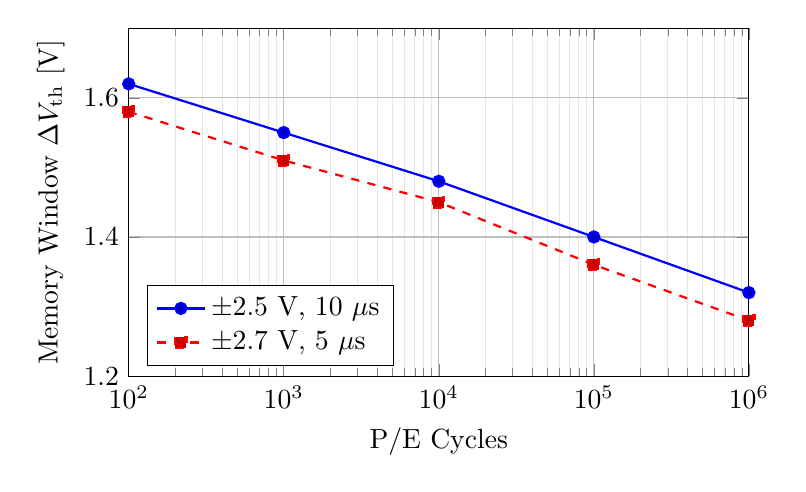
\begin{tikzpicture}
\begin{axis}[
  width=0.78\textwidth, height=60mm,
  xlabel={P/E Cycles}, xmode=log, log basis x=10,
  ylabel={Memory Window $\Delta V_\text{th}$ [V]},
  ymin=1.2, ymax=1.7, xmin=1e2, xmax=1e6,
  legend pos=south west, legend cell align=left, grid=both, minor grid style={gray!20},
  tick label style={/pgf/number format/fixed}
]
\addplot+[mark=*,thick] table[row sep=\\]{
x   y\\
1e2 1.62\\
1e3 1.55\\
1e4 1.48\\
1e5 1.40\\
1e6 1.32\\
};
\addlegendentry{$\pm$2.5 V, 10 $\mu$s}

\addplot+[mark=square*,thick,dashed] table[row sep=\\]{
x   y\\
1e2 1.58\\
1e3 1.51\\
1e4 1.45\\
1e5 1.36\\
1e6 1.28\\
};
\addlegendentry{$\pm$2.7 V, 5 $\mu$s}
\end{axis}
\end{tikzpicture}
\caption{Schematic endurance behavior of HZO-FeFETs in a 0.18\,$\mu$m flow.}
\label{fig:endurance}
\end{figure*}

\clearpage

% -------- Fig.3: Wake-up & Retention --------
\begin{figure*}[p]
\centering
\begin{minipage}{0.44\textwidth}
\centering
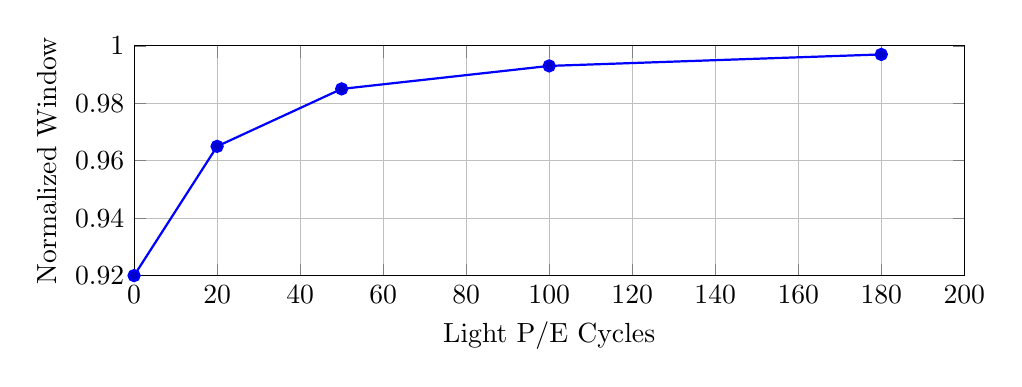
\begin{tikzpicture}
\begin{axis}[
  width=\linewidth, height=45mm,
  xlabel={Light P/E Cycles}, xmin=0, xmax=200,
  ylabel={Normalized Window}, ymin=0.92, ymax=1.00,
  grid=both, legend pos=south east
]
\addplot+[thick] table[row sep=\\]{
x y\\
0 0.92\\
20 0.965\\
50 0.985\\
100 0.993\\
180 0.997\\
};
\end{axis}
\end{tikzpicture}\\
\footnotesize (a) Wake-up (early cycles).
\end{minipage}\hfill
\begin{minipage}{0.44\textwidth}
\centering
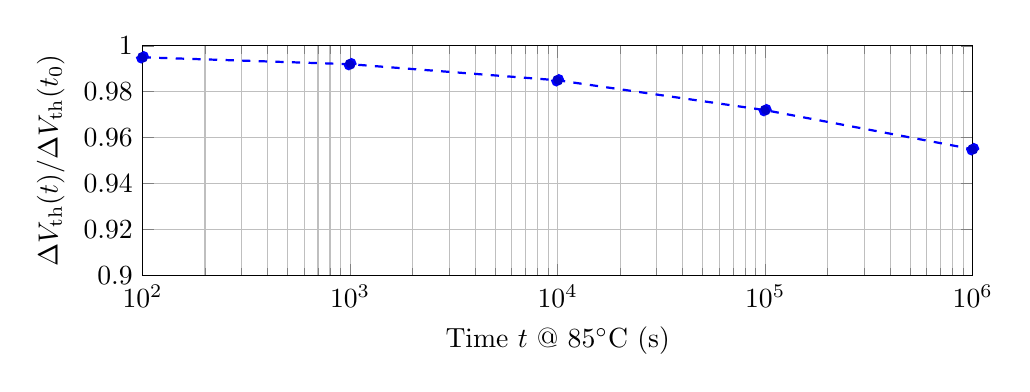
\begin{tikzpicture}
\begin{axis}[
  width=\linewidth, height=45mm,
  xlabel={Time $t$ @ 85$^\circ$C (s)}, xmode=log, xmin=1e2, xmax=1e6,
  ylabel={$ \Delta V_\text{th}(t)/\Delta V_\text{th}(t_0)$}, ymin=0.9, ymax=1.0,
  grid=both
]
\addplot+[thick,dashed] table[row sep=\\]{
x y\\
1e2 0.995\\
1e3 0.992\\
1e4 0.985\\
1e5 0.972\\
1e6 0.955\\
};
\end{axis}
\end{tikzpicture}\\
\footnotesize (b) Retention (projection).
\end{minipage}
\caption{Wake-up and retention behaviors (illustrative).}
\label{fig:wakeup}
\end{figure*}

\clearpage

% -------- Fig.4: TDDB Weibull --------
\begin{figure*}[p]
\centering
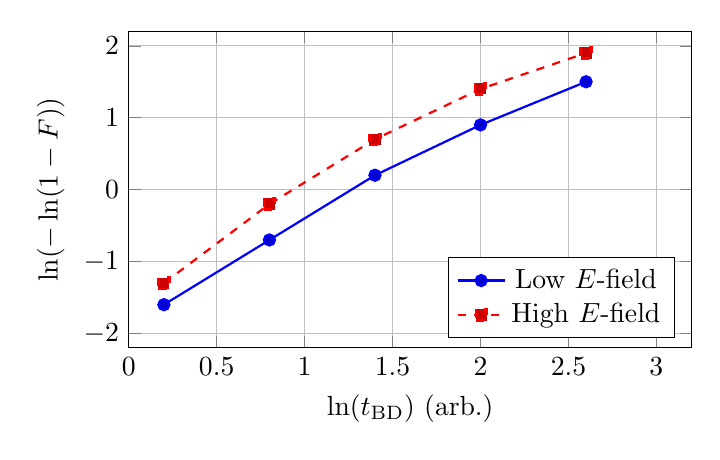
\begin{tikzpicture}
\begin{axis}[
  width=0.72\textwidth, height=56mm,
  xlabel={$\ln(t_\text{BD})$ (arb.)}, ylabel={$\ln\!\left(-\ln(1-F)\right)$},
  grid=both, legend pos=south east, ymin=-2.2, ymax=2.2, xmin=0, xmax=3.2
]
\addplot+[thick] table[row sep=\\]{
x y\\
0.2 -1.6\\
0.8 -0.7\\
1.4  0.2\\
2.0  0.9\\
2.6  1.5\\
};
\addlegendentry{Low $E$-field}
\addplot+[thick,dashed,mark=square*] table[row sep=\\]{
x y\\
0.2 -1.3\\
0.8 -0.2\\
1.4  0.7\\
2.0  1.4\\
2.6  1.9\\
};
\addlegendentry{High $E$-field}
\end{axis}
\end{tikzpicture}
\caption{TDDB Weibull representation at two stress fields (illustrative).}
\label{fig:tddb}
\end{figure*}

\end{document}
